\chapter{Marco Teórico}
%\epigraph{\textit{Research is what I'm doing when I don't know what I'm doing.   
%	}}{\textit{— Wernher von Braun, NASA engineer}}
%	\vspace*{8cm}
%	\begin{center}
%		\centering
%		\includegraphics[width=10.5cm]{example-image}
 %   \end{center}
%\thispagestyle{empty}
%\newpage
\vspace*{2cm}
En este capítulo abordaremos algunos temas y conceptos teóricos para sentar la base necesaria del proyecto y de este modo, continuar con el diseño del proyecto.

\section{Algoritmos de predicción}
En uno de los trabajos de Galam, propone una población que evoluciona a través de un contexto con dos opciones con una probabilidad de éxito o fracaso, de un espacio de individuos cualquiera y de este espacio, dividirlos en 3 grupos generando una nueva población para evaluar a la mayoría predominante en esas particiones. \cite{Galam2008}
% Insertar diagrama del TT

En los grupos no es estrictamente necesario ser de 3 individuos, el agrupamiento de individuos puede ser de cualquier tamaño, este comportamiento puede aplicarse a distintos casos, ya que es posible evaluar el desarrollo de un comportamiento de la población.

\subsection{Modelo de reglas de la mayoría local}
Consideramos grupos, que están constituidos por la segregación aleatoria de 3 agentes. Da la probabilidad de tener un \textbf{A} elegido en el nivel \textit{(n + 1)} de un grupo de nivel \textit{n} donde $P_{n}$ es la porción de personas \textbf{A} elegidas en el n-nivel.\cite{Galam2008}
\begin{equation}
    p_{n}+1 \equiv P_{3}(p_{n}) = p_{n}^3 + 3p_{n}^2(1-p_{n})
\end{equation}
La función de votación $P_{3}(p_{n})$ tiene 3 puntos fijos $p_{d} = 0$, $p_{c,3} = 1/2$ y $p_{t} = 1$. El primero corresponde a la desaparición de A. El último punto $p_{t}$ representa la situación de la dictadura donde solo \textbf{A} esta presente. Ambos son estables. Por el contrario, $p_{c}$ es inestable. Para determinar el umbral a plena potencia. A partir de $p_{0} < 1/2$ la votación repetida conduce a (0) mientras que el flujo esta en la dirección de (1) para $p_{0} > 1/2$.\cite{Galam2008}

\begin{figure}[!ht]
    \centering
    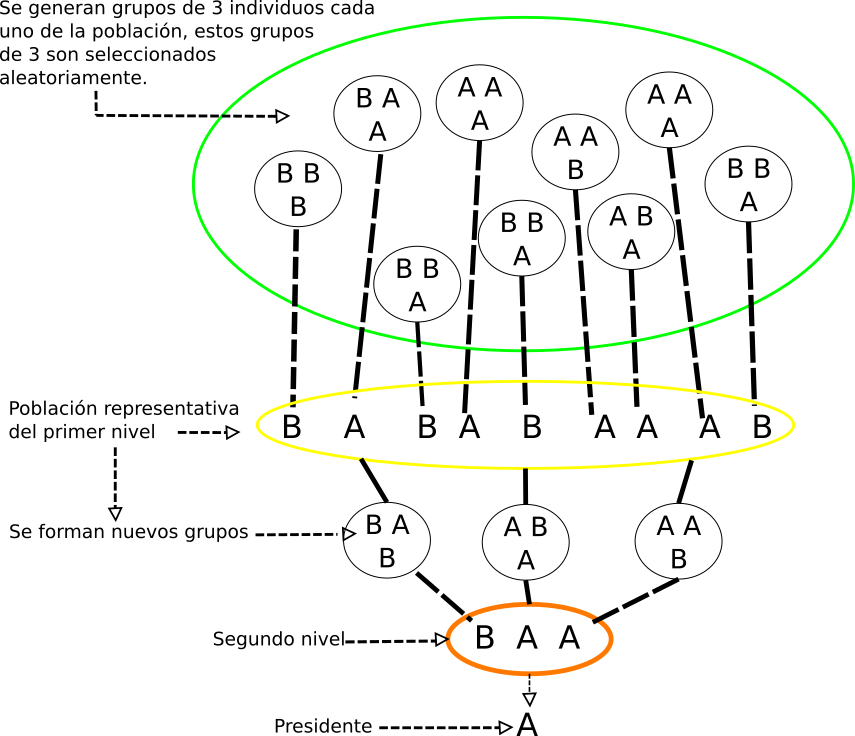
\includegraphics[scale=0.50]{TT/img/marco teorico/prediccion.png}
    \caption{Jerarquización de la población a través de diferentes iteraciones}
    \label{graphic:prediccion}
\end{figure}

Por lo tanto, la votación por regla de la mayoría produce la auto-eliminación de cualquier proporción de la tendencia \textbf{A}, mientras que $p_{0} < 1/2$, siempre que exista un número suficiente de votación, esto lo vemos en la figura \ref{graphic:prediccion}. Por consiguiente, es esencial determinar el número de niveles necesarios para garantizar el liderazgo completo a la mayor tendencia inicial. \cite{Galam2008}
%Insertar imagen describiendo el funcionamiento del algoritmo

\subsection{Grupos de votación mas grandes y la fórmula mágica}
Para grupos de votación de cualquier tamaño \textbf{\textit{r}} la función de votación $p_{n+1} = P_{r}(p_{n})$ se escribe:
\begin{equation}
    P_{r}(p_{n}) = \sum_{l=r}^{l=m} \frac{r!}{l!(r-l)!}p_{n}^{l}(1+p_{n})^{r-l},
\end{equation}
donde $m = (r + 1)/2$ para r impar y $m = (r + 1)/2$ para r par para dar cuenta del sesgo favorecido por \textbf{B}. Los dos puntos fijos estables $p_{d} = 0$ y $p_{t} = 1$ son independientes del tamaño del grupo \textbf{\textit{r}}. La inestable $p_{c,r} = 1/2$ también es independiente del tamaño del grupo \textbf{\textit{r}} para valores impares de r, para los cuales no existe sesgo. Por el contrario, varía con \textbf{\textit{r}} para valores pares. Comienza en $p_{c,2} = 1$ para $r = 2$, disminuye a $p_{c,4} = (1 + \sqrt{13})/6 \approx 0.77$ para $\textbf{\textit{r}} = 4$ y luego sigue disminuyendo asintóticamente hacia $1/2$ desde arriba.

